\documentclass[12pt]{article} % Default font size is 12pt, it can be changed here

    \usepackage{geometry} % Required to change the page size to A4
    \geometry{a4paper} % Set the page size to be A4 as opposed to the default US Letter
    
    \usepackage{graphicx} % Required for including pictures

    \usepackage{mathtools, nccmath}
    
    \usepackage{tikz}
    \usetikzlibrary{matrix,calc}

    %isolated term
%#1 - Optional. Space between node and grouping line. Default=0
%#2 - node
%#3 - filling color
\newcommand{\implicantsol}[3][0]{
    \draw[rounded corners=3pt, fill=#3, opacity=0.3] ($(#2.north west)+(135:#1)$) rectangle ($(#2.south east)+(-45:#1)$);
    }


%internal group
%#1 - Optional. Space between node and grouping line. Default=0
%#2 - top left node
%#3 - bottom right node
%#4 - filling color
\newcommand{\implicant}[4][0]{
    \draw[rounded corners=3pt, fill=#4, opacity=0.3] ($(#2.north west)+(135:#1)$) rectangle ($(#3.south east)+(-45:#1)$);
    }

%group lateral borders
%#1 - Optional. Space between node and grouping line. Default=0
%#2 - top left node
%#3 - bottom right node
%#4 - filling color
\newcommand{\implicantcostats}[4][0]{
    \draw[rounded corners=3pt, fill=#4, opacity=0.3] ($(rf.east |- #2.north)+(90:#1)$)-| ($(#2.east)+(0:#1)$) |- ($(rf.east |- #3.south)+(-90:#1)$);
    \draw[rounded corners=3pt, fill=#4, opacity=0.3] ($(cf.west |- #2.north)+(90:#1)$) -| ($(#3.west)+(180:#1)$) |- ($(cf.west |- #3.south)+(-90:#1)$);
}

%group top-bottom borders
%#1 - Optional. Space between node and grouping line. Default=0
%#2 - top left node
%#3 - bottom right node
%#4 - filling color
\newcommand{\implicantdaltbaix}[4][0]{
    \draw[rounded corners=3pt, fill=#4, opacity=0.3] ($(cf.south -| #2.west)+(180:#1)$) |- ($(#2.south)+(-90:#1)$) -| ($(cf.south -| #3.east)+(0:#1)$);
    \draw[rounded corners=3pt, fill=#4, opacity=0.3] ($(rf.north -| #2.west)+(180:#1)$) |- ($(#3.north)+(90:#1)$) -| ($(rf.north -| #3.east)+(0:#1)$);
}

%group corners
%#1 - Optional. Space between node and grouping line. Default=0
%#2 - filling color
\newcommand{\implicantcantons}[2][0]{
    \draw[rounded corners=3pt, opacity=.3] ($(rf.east |- 0.south)+(-90:#1)$) -| ($(0.east |- cf.south)+(0:#1)$);
    \draw[rounded corners=3pt, opacity=.3] ($(rf.east |- 8.north)+(90:#1)$) -| ($(8.east |- rf.north)+(0:#1)$);
    \draw[rounded corners=3pt, opacity=.3] ($(cf.west |- 2.south)+(-90:#1)$) -| ($(2.west |- cf.south)+(180:#1)$);
    \draw[rounded corners=3pt, opacity=.3] ($(cf.west |- 10.north)+(90:#1)$) -| ($(10.west |- rf.north)+(180:#1)$);
    \fill[rounded corners=3pt, fill=#2, opacity=.3] ($(rf.east |- 0.south)+(-90:#1)$) -|  ($(0.east |- cf.south)+(0:#1)$) [sharp corners] ($(rf.east |- 0.south)+(-90:#1)$) |-  ($(0.east |- cf.south)+(0:#1)$) ;
    \fill[rounded corners=3pt, fill=#2, opacity=.3] ($(rf.east |- 8.north)+(90:#1)$) -| ($(8.east |- rf.north)+(0:#1)$) [sharp corners] ($(rf.east |- 8.north)+(90:#1)$) |- ($(8.east |- rf.north)+(0:#1)$) ;
    \fill[rounded corners=3pt, fill=#2, opacity=.3] ($(cf.west |- 2.south)+(-90:#1)$) -| ($(2.west |- cf.south)+(180:#1)$) [sharp corners]($(cf.west |- 2.south)+(-90:#1)$) |- ($(2.west |- cf.south)+(180:#1)$) ;
    \fill[rounded corners=3pt, fill=#2, opacity=.3] ($(cf.west |- 10.north)+(90:#1)$) -| ($(10.west |- rf.north)+(180:#1)$) [sharp corners] ($(cf.west |- 10.north)+(90:#1)$) |- ($(10.west |- rf.north)+(180:#1)$) ;
}

%Empty Karnaugh map 4x4
\newenvironment{Karnaugh}%
{
\begin{tikzpicture}[baseline=(current bounding box.north),scale=0.8]
\draw (0,0) grid (4,4);
\draw (0,4) -- node [pos=0.7,above right,anchor=south west] {AB} node [pos=0.75,below left,anchor=north east] {CD} ++(135:1);
%
\matrix (mapa) [matrix of nodes,
        column sep={0.8cm,between origins},
        row sep={0.8cm,between origins},
        every node/.style={minimum size=0.3mm},
        anchor=8.center,
        ampersand replacement=\&] at (0.5,0.5)
{
                       \& |(c00)| 00         \& |(c01)| 01         \& |(c11)| 11         \& |(c10)| 10         \& |(cf)| \phantom{00} \\
|(r00)| 00             \& |(0)|  \phantom{0} \& |(1)|  \phantom{0} \& |(3)|  \phantom{0} \& |(2)|  \phantom{0} \&                     \\
|(r01)| 01             \& |(4)|  \phantom{0} \& |(5)|  \phantom{0} \& |(7)|  \phantom{0} \& |(6)|  \phantom{0} \&                     \\
|(r11)| 11             \& |(12)| \phantom{0} \& |(13)| \phantom{0} \& |(15)| \phantom{0} \& |(14)| \phantom{0} \&                     \\
|(r10)| 10             \& |(8)|  \phantom{0} \& |(9)|  \phantom{0} \& |(11)| \phantom{0} \& |(10)| \phantom{0} \&                     \\
|(rf) | \phantom{00}   \&                    \&                    \&                    \&                    \&                     \\
};
}%
{
\end{tikzpicture}
}

%Empty Karnaugh map 2x4
\newenvironment{Karnaughvuit}%
{
\begin{tikzpicture}[baseline=(current bounding box.north),scale=0.8]
\draw (0,0) grid (4,2);
\draw (0,2) -- node [pos=0.7,above right,anchor=south west] {bc} node [pos=0.7,below left,anchor=north east] {a} ++(135:1);
%
\matrix (mapa) [matrix of nodes,
        column sep={0.8cm,between origins},
        row sep={0.8cm,between origins},
        every node/.style={minimum size=0.3mm},
        anchor=4.center,
        ampersand replacement=\&] at (0.5,0.5)
{
                      \& |(c00)| 00         \& |(c01)| 01         \& |(c11)| 11         \& |(c10)| 10         \& |(cf)| \phantom{00} \\
|(r00)| 0             \& |(0)|  \phantom{0} \& |(1)|  \phantom{0} \& |(3)|  \phantom{0} \& |(2)|  \phantom{0} \&                     \\
|(r01)| 1             \& |(4)|  \phantom{0} \& |(5)|  \phantom{0} \& |(7)|  \phantom{0} \& |(6)|  \phantom{0} \&                     \\
|(rf) | \phantom{00}  \&                    \&                    \&                    \&                    \&                     \\
};
}%
{
\end{tikzpicture}
}

%Empty Karnaugh map 2x2
\newenvironment{Karnaughquatre}%
{
\begin{tikzpicture}[baseline=(current bounding box.north),scale=0.8]
\draw (0,0) grid (2,2);
\draw (0,2) -- node [pos=0.7,above right,anchor=south west] {b} node [pos=0.7,below left,anchor=north east] {a} ++(135:1);
%
\matrix (mapa) [matrix of nodes,
        column sep={0.8cm,between origins},
        row sep={0.8cm,between origins},
        every node/.style={minimum size=0.3mm},
        anchor=2.center,
        ampersand replacement=\&] at (0.5,0.5)
{
          \& |(c00)| 0          \& |(c01)| 1  \\
|(r00)| 0 \& |(0)|  \phantom{0} \& |(1)|  \phantom{0} \\
|(r01)| 1 \& |(2)|  \phantom{0} \& |(3)|  \phantom{0} \\
};
}%
{
\end{tikzpicture}
}

%Defines 8 or 16 values (0,1,X)
\newcommand{\contingut}[1]{%
\foreach \x [count=\xi from 0]  in {#1}
     \path (\xi) node {\x};
}

%Places 1 in listed positions
\newcommand{\minterms}[1]{%
    \foreach \x in {#1}
        \path (\x) node {1};
}

%Places 0 in listed positions
\newcommand{\maxterms}[1]{%
    \foreach \x in {#1}
        \path (\x) node {0};
}

%Places X in listed positions
\newcommand{\indeterminats}[1]{%
    \foreach \x in {#1}
        \path (\x) node {X};
}

    \linespread{1.2} % Line spacing
    
    \setlength\parindent{0pt} % Uncomment to remove all indentation from paragraphs
    
    \graphicspath{{/home/bzerol/VisualCode/ElectroIII/tp1-team-2/E2TP1}} % Specifies the directory where pictures are stored

    
    
    \begin{document}

    \section{Exercise 2} % Major section
    
    Having the function in maxterms $$f_1 (A,B,C,D) = \prod\left(M_0, M_1 , M_5 , M_7 , M_8 , M_{10} , M_{14} , M_{15} \right)$$ equivalent to $$f_2 (A,B,C,D) = \sum\left(m_2, m_3 , m_4 , m_6 , m_9 , m_{11} , m_{12} , m_{13} \right)$$ using minterms, can be simplify by different ways and represented using logic gates.

    \subsection{Simplify: Boolean Algebra}

    Using the Boolean algebra propertie $$(A+B).(A+\overline{B})=A~(1)$$ or $$(AB)+(A\overline{B})=A~(2)$$ the function could be simplify using (1): 
    \begin{eqnarray*}
        f_1 (A,B,C,D) &= &(A+B+C+D).(A+B+C+\overline{D}).(A+\overline{B}+C+\overline{D}).(A+\overline{B}+\overline{C}+\overline{D}).\\
        &&(\overline{A}+B+C+D).(\overline{A}+B+\overline{C}+D).(\overline{A}+\overline{B}+\overline{C}+D).(\overline{A}+\overline{B}+\overline{C}+\overline{D}) \\
        &=&(A+B+C).(A+\overline{B}+\overline{D}).(\overline{A}+B+D).(\overline{A}+\overline{B}+\overline{C})
    \end{eqnarray*}
    Which in minterms would be, using (2):
    \begin{eqnarray*}
        f_2(A,B,C,D) &= &(\overline{A}\overline{B}C\overline{D})+(\overline{A}\overline{B}CD)+(\overline{A}B\overline{C}\overline{D})+(\overline{A}BC\overline{D})+\\
        &&(A\overline{B}\overline{C}D)+(A\overline{B}CD)+(AB\overline{C}\overline{D})+(AB\overline{C}D)\\
        &=&(A\overline{B}D)+(\overline{A}B\overline{D})+(\overline{A}\overline{B}C)+(AB\overline{C})
    \end{eqnarray*}

    \subsection{Simplify: Karnaugh Map}

    Karnaugh map is a easier way to simplify logic experesion when the functions are too complex or too large to handle, cause Karnaugh map gives a more representative view for a faster analisis for it to simplify. 

    If the simplification is done with minterms, the groups should be of $1$, adding each group in case there is more than 1, and in each group the independent variables would be multiplied.
    \begin{center}
        \begin{Karnaugh}
            %cada 4 es una fila, la col 3 es la 4ta columna y 3fila es la 4 fila
            \contingut{
            0,1,0,1,
            0,0,1,1,
            1,1,0,0,
            1,0,1,0} 
            \implicant{6}{14}{red}
            \implicant{3}{7}{green}
            \implicant{12}{8}{orange}
            \implicantdaltbaix[3pt]{1}{9}{blue}
            %\implicantcantons[2pt]{orange}
            %\implicantcostats{4}{14}{green}
        \end{Karnaugh}
    \end{center}
    
    Now grouping the colour groups we get that the function in minterms would be:
    \begin{eqnarray*}
        f_2(A,B,C,D)&=&(A\overline{B}D)~(Red)\\
        &&+(\overline{A}B\overline{D})~(Blue)\\
        &&+(\overline{A}\overline{B}C)~(Orange)\\
        &&+(AB\overline{C})~(Green)
    \end{eqnarray*}
 
    The same method could be done with maxterms; grouping $O$, multipling groups in case there is more than 1, and in each group the independent variables would be added.
    
    \subsection{Logic Circuit: AND, OR and NOT}

    Using the logic gates AND, OR and NOT the simplify version of the function could be represented in the figure below:

    \begin{figure}[htb!]
        \centering
        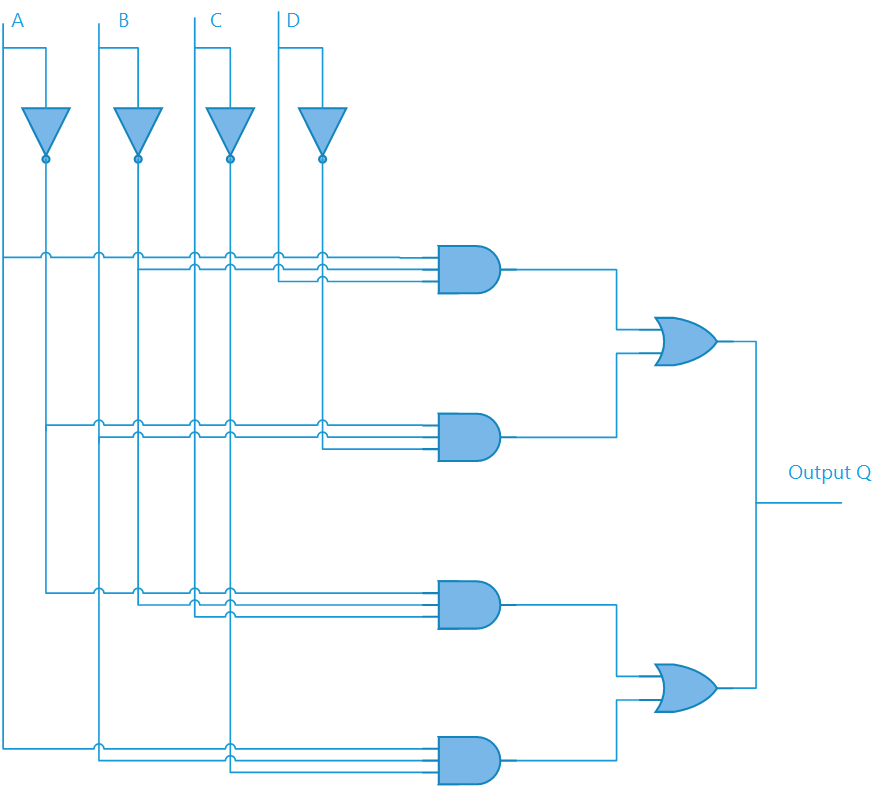
\includegraphics[scale=0.45]{normallogic.png}
        \caption{Logic circuit using AND, OR and NOT gates}
        \label{fig:normllogic}
    \end{figure}
    
    \pagebreak

    \subsection{Logic Circuit: NAND}

    All the gates could be equivalent to a combination of NAND or NOR gates. Therefore, the simplify function can be drawn as the next figure:

    \begin{figure}[h!]
        \centering
        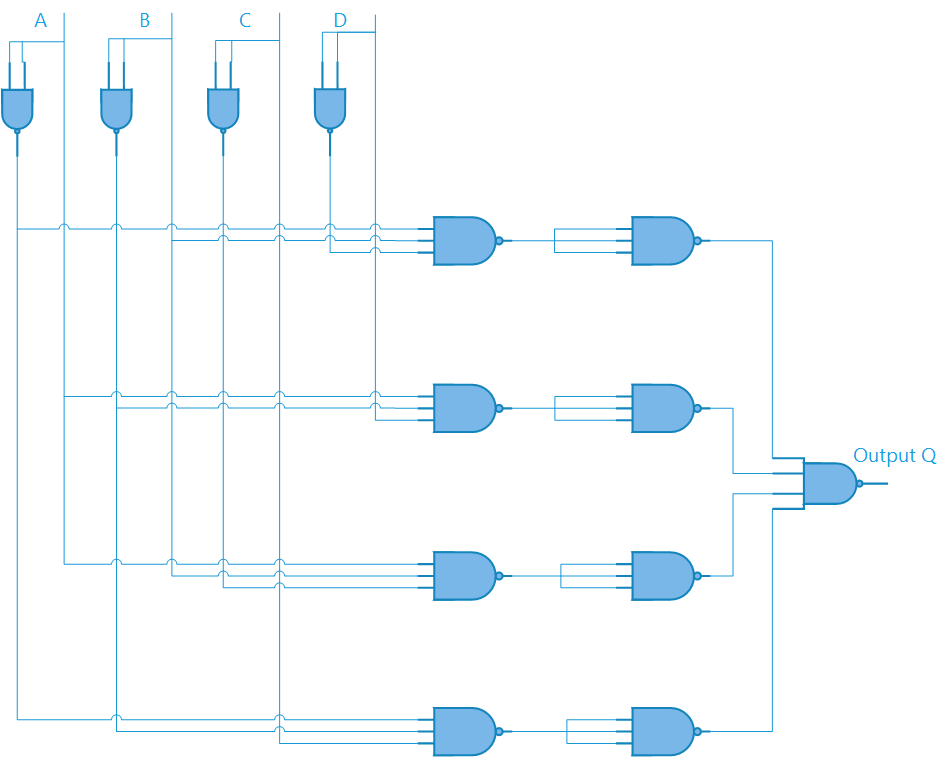
\includegraphics[scale=0.45]{nandlogic.png}
        \caption{Logic circuit using NAND gates}
        \label{fig:nandlogic}
    \end{figure}


    \end{document}